
%-----------------------------------------------%

% PREAMBLE %

%-----------------------------------------------%
\documentclass[a4paper,12pt]{article}

% Packages
\usepackage{textcomp}
\usepackage{gensymb}
\usepackage{graphicx}
\usepackage{amsmath}
\usepackage{geometry}
\usepackage{fancyhdr}
\usepackage{setspace}
\usepackage{titlesec}  % For title formatting
\usepackage{tocloft}
\usepackage{xcolor}
\usepackage{enumitem}


% Header and Footer
\pagestyle{fancy}
\fancyhf{}
\fancyhead[L]{Abereni Opuiyo}
\fancyhead[C]{PHY121}
\fancyhead[R]{\thepage}
\fancyfoot[L]{Final Project: Physics Illustrated in "Hancock"}
\fancyfoot[R]{\nouppercase{\rightmark}}
\geometry{margin=1.2in}
\setstretch{1.5}


\newcommand*{\justifyheading}{\raggedleft}
\renewcommand{\sectionmark}[1]{\markright{#1}}
\renewcommand{\footrulewidth}{0.1pt}% default is 0pt

% Table of Contents
\renewcommand{\contentsname}{Table of Contents}
\renewcommand{\cftsecleader}{\cftdotfill{\cftdotsep}}



% Title Formatting

\titleformat{\section}
	{\normalfont\huge\bfseries\justifyheading}
	{\thesection}
	{1em}{}
	

\titleformat{\subsection}
	{\normalfont\Large\bfseries}
	{\thesubsection}
	{1em}{}
	[{\titlerule[1.8pt]}]

% Cover Page
\title{
    \vspace{5cm} % Adjust vertical space
    
\includegraphics[width=0.55\textwidth]{dutchess-logo-blue.png} \\ % Add your logo here (change "logo.png" to the actual filename)
    \vspace{1cm} % Adjust vertical space after the logo
    \textbf{\Huge Final Project: Physics Illustrated in "Hancock"} \\
    \vspace{1cm} % Adjust vertical space
    \large PHY121 \\
    \vspace{0.5cm} % Adjust vertical space
    \large	October, 4th, 2024 \\ 
		\vspace{.5cm}
		\large Professor Renee Lathrop 
}
\author{Abereni Opuiyo}
\date{}
%-----------------------------------------------%

% TITLE PAGE %

%-----------------------------------------------%
\begin{document}
\maketitle
	\thispagestyle{plain}
\newpage

%-----------------------------------------------%

% Table of Contents  %

%-----------------------------------------------%
% Start page numbering from the Table of Contents

\setcounter{secnumdepth}{0}
\setcounter{page}{1}  % Start counting from 1
\tableofcontents
\thispagestyle{fancy}
\newpage

%-----------------------------------------------%
\section{Unit 1}

\vspace{-0.5cm}
\singlespacing

\subsection{Scene Analysis}

\textbf{Duration}: 25:40 - 27:55

\vspace{0.3cm}
\noindent\textbf{Summary:} \par
On the first day of trying to reform his public image, the superhero Hancock loses his temper to a 10 year old child and throws them a couple hundred meters into the air. After a couple seconds, Hancock catches them right before they touch the ground. \par


\vspace{0.3cm}
\noindent\textbf{Concepts Demonstrated} \par
I think this scene covers many aspects of \textit{kinematics} well, including \textit{projectile motion}, \textit{acceleration due to gravity}, and \textit{free falling bodies}. 

\subsection{Problem 1}

If Hancock throws the child at an angle of 80\degree\ and an initial velocity of $60\ {m/s}$, how long does it take for the child to reach their maximum height in the air?

\subsubsection{Solution:}

\begin{figure}[h]
    \centering
    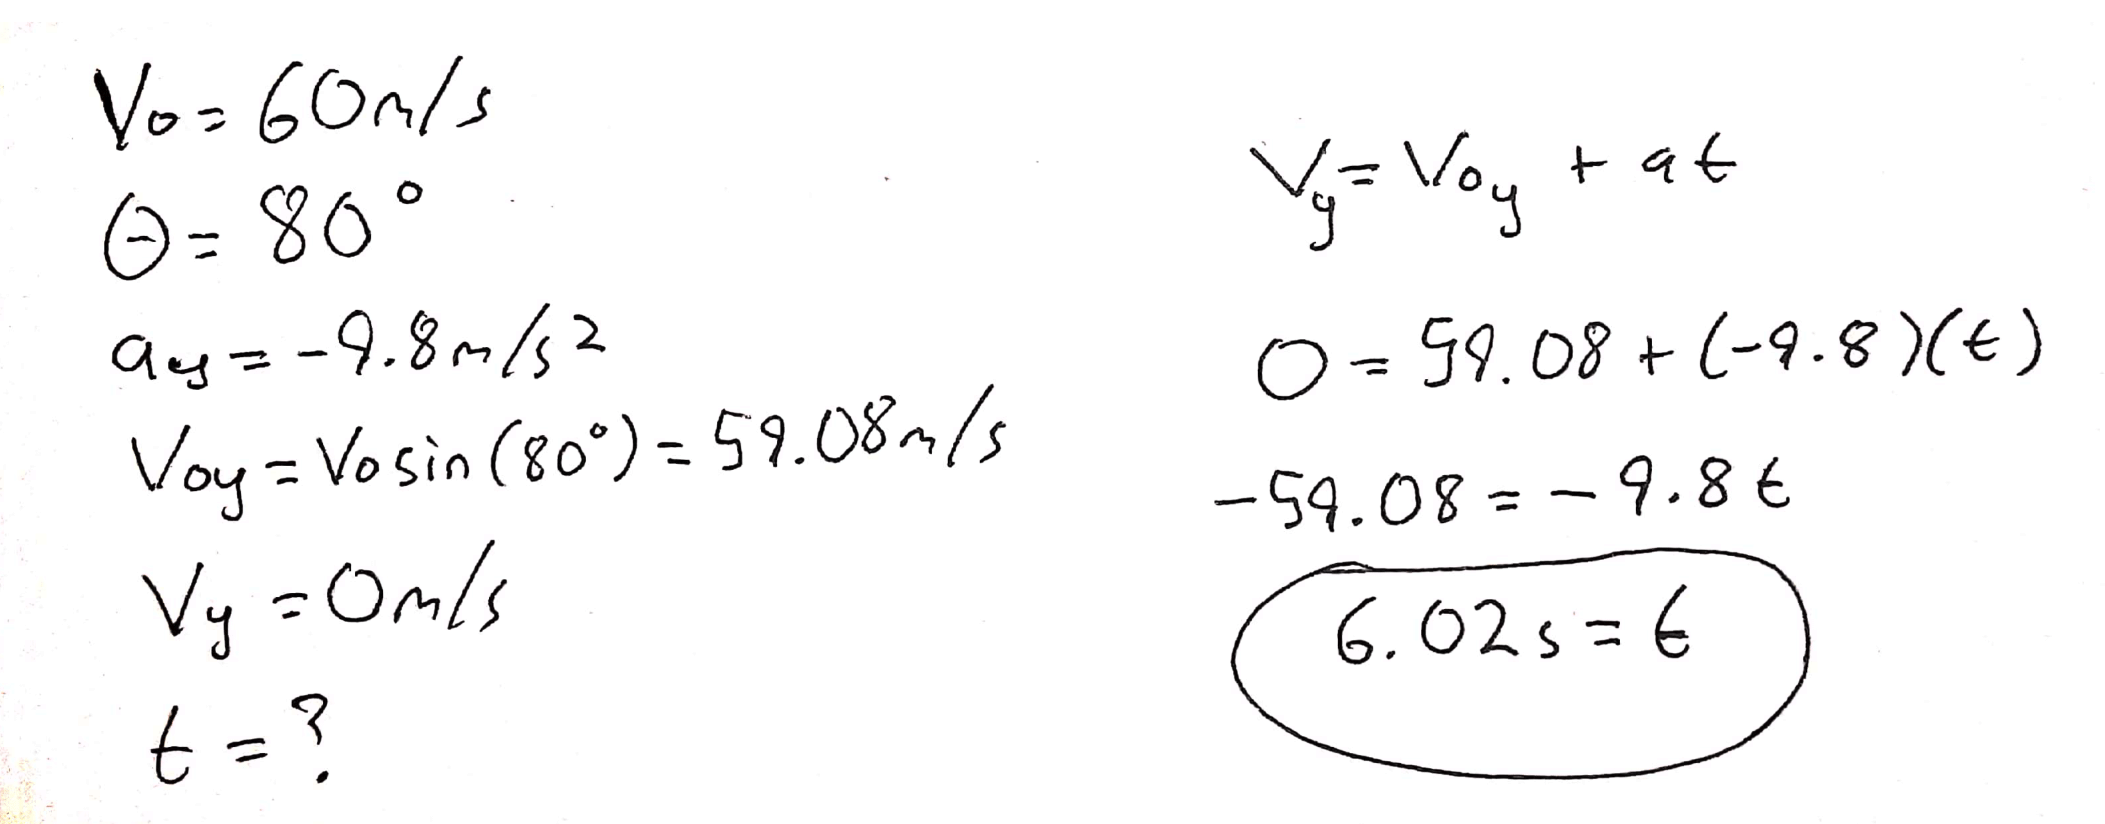
\includegraphics[width=0.8\textwidth]{U1P1S} % Example of adding a figure
\end{figure}

\newpage

\subsection{Problem 2}

Using the answer you got from Problem 1, calculate how far Hancock will have to walk to catch the child and avoid a longer jail sentence.

\subsubsection{Solution:}

\begin{figure}[h]
    \centering
    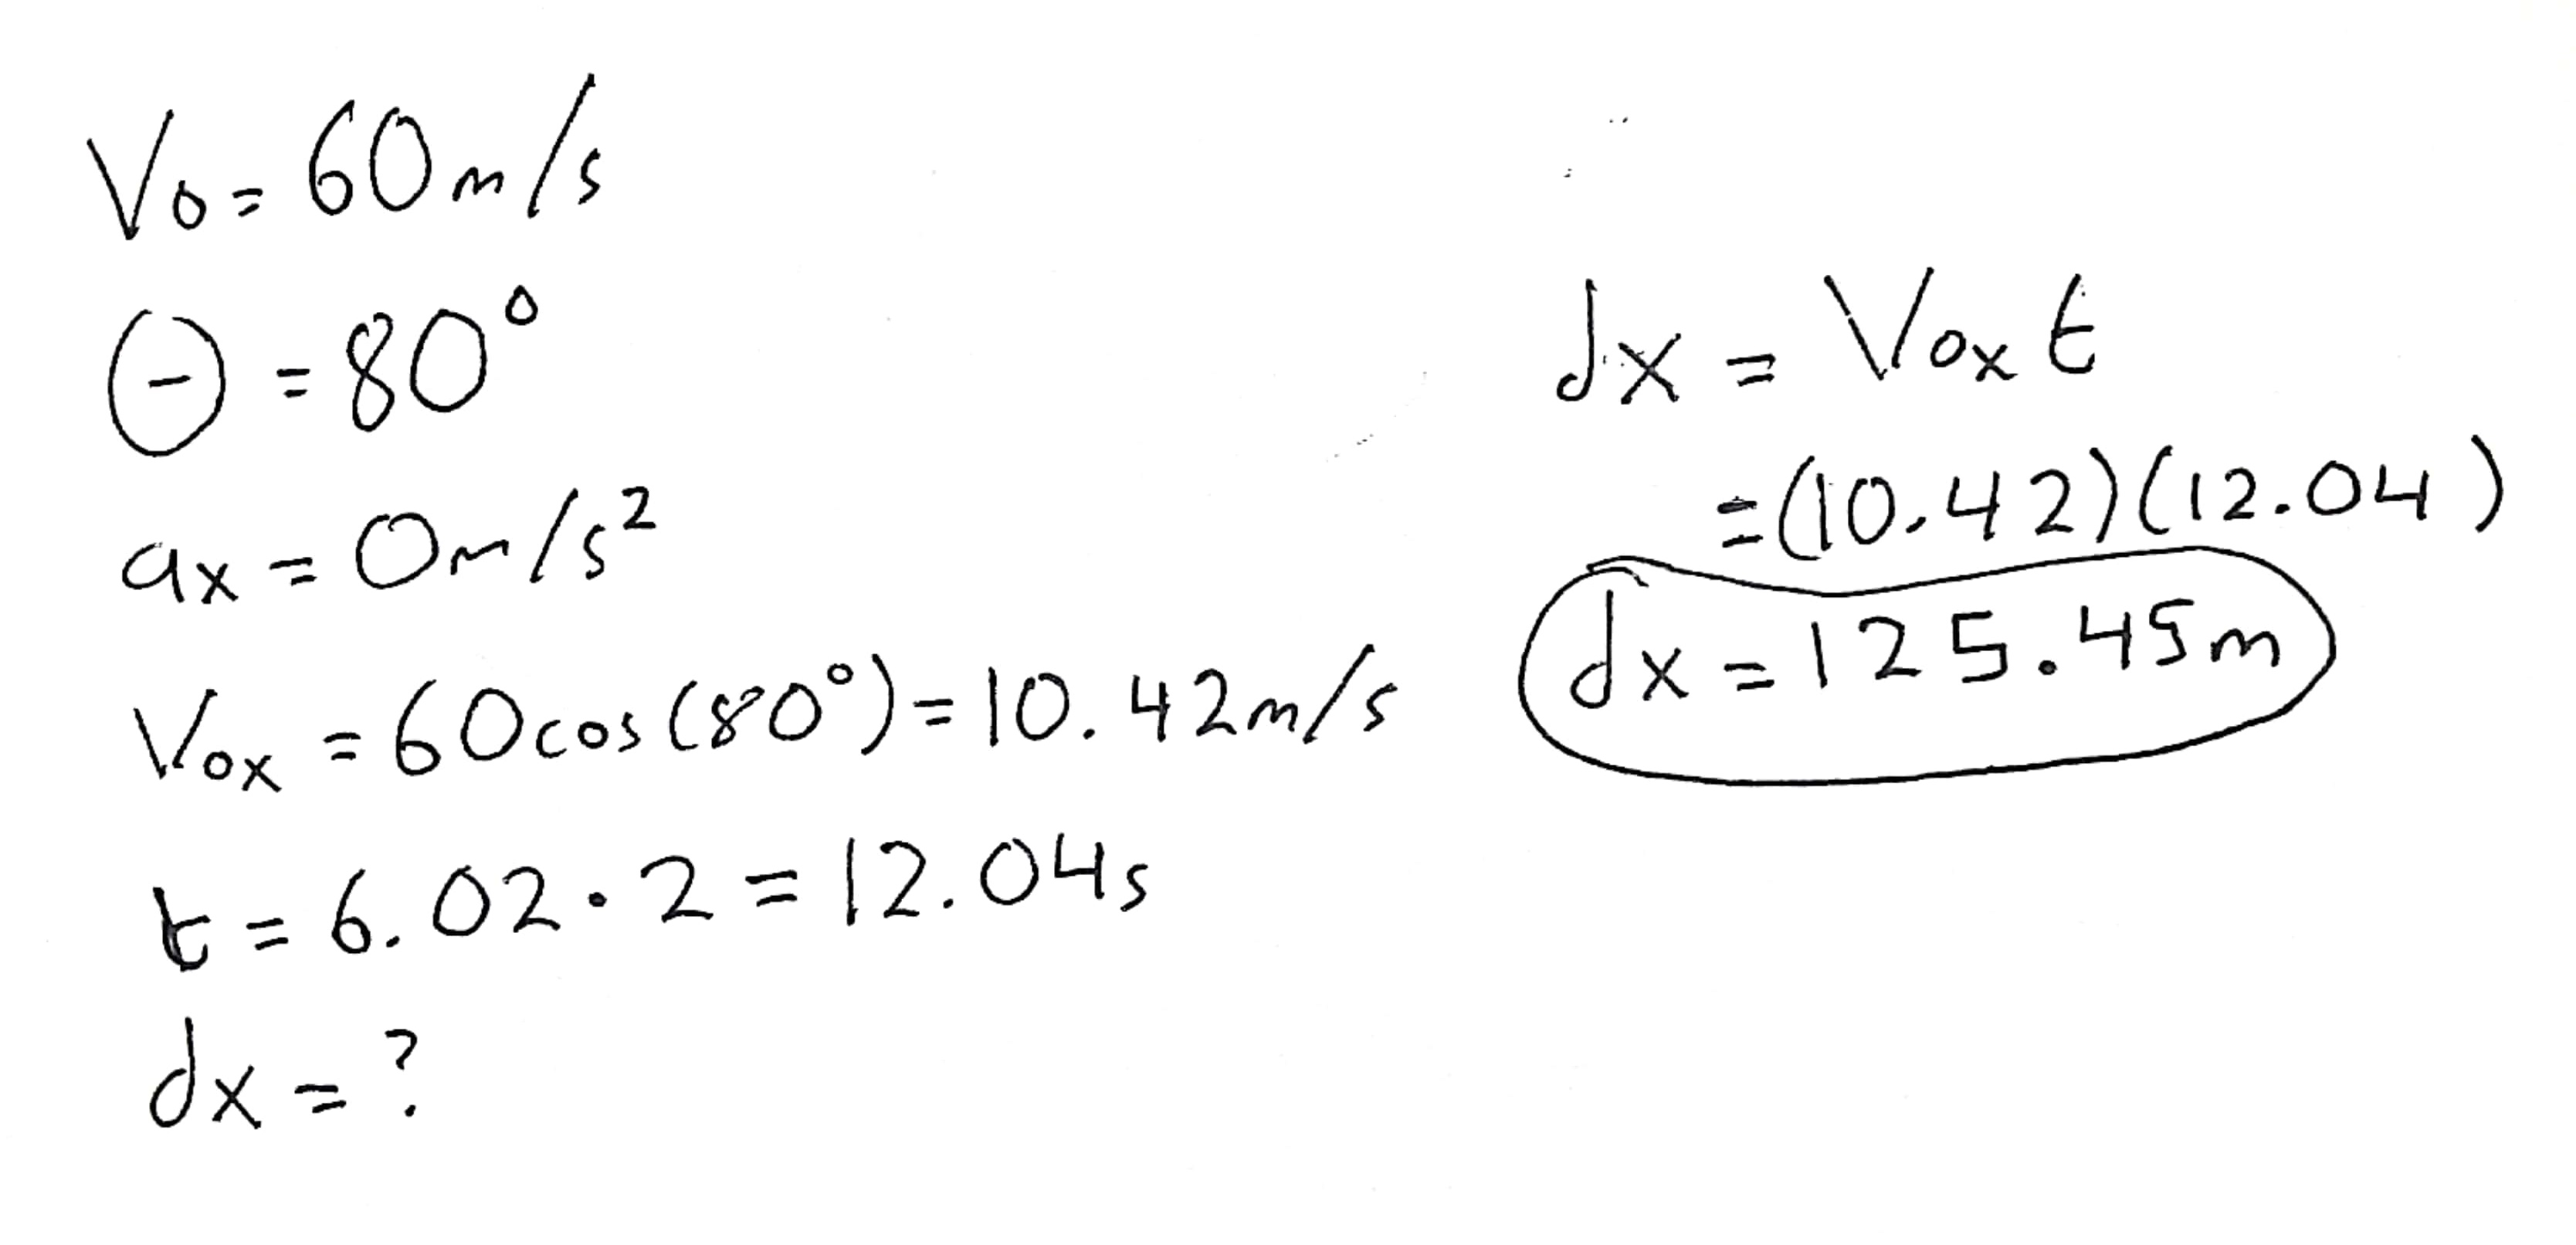
\includegraphics[width=0.8\textwidth]{U1P2S} % Example of adding a figure
\end{figure}

\end{document}
